\cleardoublepage
\chapter{基于共识协议的节点选择机制}
\label{sec:consensus}
确定最佳的存储节点选择是构建高效区块链存储系统的关键一环。
根据本文测量中的分析,如图\autoref{fig:dis_cdf}所示,存储节点与网关之间的距离对数据访问延迟有着直接的影响。
此外,在链下存储环境中,节点存储空间不足或恶意行为可能会导致数据的丢失、被篡改或服务中断,这些都会对系统的安全性和稳定性造成严重影响。
因此,如何选择最佳的存储节点是一个挑战。

\section{中心化节点选择}
在区块链和分布式存储系统中,存储节点的选择是确保数据安全性和可靠性的关键步骤。
目前,许多系统如Storj~\cite{storj2018storj}、CoopEdge~\cite{yuan2021coopedge}和PipeEdge~\cite{yuan2023pipeedge}根据节点的信誉选择存储节点,通过区块链来确认节点选择的决策。
鉴于PBFT共识算法在分布式系统中的普遍应用,本文将阐述一个基于PBFT算法的去中心化存储系统中节点选择的具体步骤和流程。
对于一个具有$3f+1$个节点的网络中,PBFT共识协议要求至多存在$f$个恶意节点。

\begin{figure}[t]
    \centering
    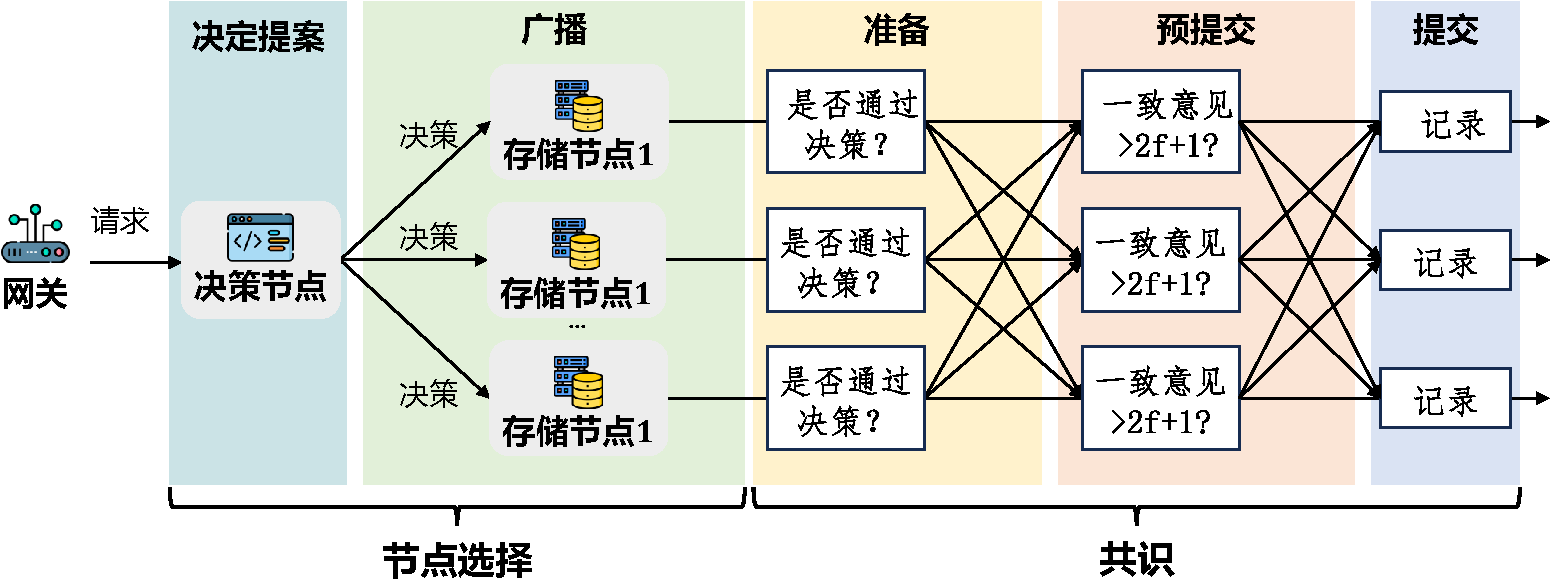
\includegraphics[width=1\linewidth]{figures/timechain/pbft.pdf}
    \caption{中心化节点选择的工作流}
    \label{fig:pbft}
\end{figure}

如\autoref{fig:pbft}所示,中心化节点选择的流程如下:
\begin{itemize}
    \item \textbf{决定提案}:
    由一个或一组节点负责评估网络中各个存储节点的信誉,根据节点的历史表现、可靠性和性能指标等因素,选择出适合承担数据存储任务的节点。
    这一阶段的目标是确保所选节点不仅具备良好的性能,还能在可靠性方面提供足够的保障。
    \item \textbf{广播}:
    决策节点(组)将最佳存储节点的提案广播给$3f+1$个存储节点。
    这一广播过程确保了所有参与节点都能接收到提案信息,为后续的共识过程奠定了基础。
    \item \textbf{准备}:
    每个存储节点决策是否通过最佳存储节点的提案,并将决策结果广播给其他的存储节点。
    这一阶段允许每个节点基于自身对提案的评估,表达对提案的支持或反对意见。
    \item \textbf{预提交}:
    当每个节点收到大于$2f+1$个相同信息(是否通过提案)时,视作该节点与其他节点的信息充分交流,并将综合的投票结果广播给其他存储节点。
    这一阶段的目的是通过节点间的通信,达成初步的共识。
    \item \textbf{提交}:
    当每个节点收到$2f+1$个信息时,选择多数一致的决策记录上链。
    由于该网络中最多存在$f$个恶意节点,因此该阶段的决策中,虚假信息的数量一定少于诚实信息,所以该系统并不会受到恶意节点的威胁。
    这种设计确保了系统能够有效抵御恶意节点的攻击,保证了节点选择过程的安全性和可靠性。
\end{itemize}

在这样的节点选择流程中,中心化节点选择引入了单点故障的风险,即如果中心节点发生故障或被恶意攻击,整个系统的节点选择和数据存储过程可能会受到影响,导致服务中断或数据丢失。
同时,这种中心化的节点选择也会导致系统的扩展性受限。
随着网络节点数量的增加,中心节点需要处理的信息量也会增加,这可能导致选择过程的延迟增加,影响整个系统的响应速度。
中心节点的计算和存储能力可能成为系统的瓶颈,限制了系统处理大规模数据的能力。

而且,共识形成过程与节点选择过程完全分离会使系统的安全性会受到威胁。
这是因为,共识过程负责确保所有节点对数据状态达成一致,而节点选择过程决定了哪些节点参与到共识中。
如果这两个过程分离,恶意节点可能利用这一点来破坏系统的安全性,例如通过选择不可靠的节点参与共识过程,从而影响数据的完整性。

\section{结合共识的节点选择过程}

\begin{algorithm}[tbp]
	\caption{Consensus Mechanism}
	\label{algo:consensus}
	\SetKwProg{Fn}{Stage}{:}{}
	\SetKwFunction{FPrepare}{准备阶段}{}
	\SetKwFunction{FPreCommit}{预提交阶段}{}
	\SetKwFunction{FComit}{提交阶段}{}
	\DontPrintSemicolon
	\SetAlgoLined
    \Fn{\FPrepare}{
        $request \gets \textit{receive}(REQUEST)$\;
        \If{$request$ 有效}{
            $d_i \gets \textit{distance}(i.pos, request.pos)$ //计算节点$i$和请求节点之间的距离\;
            $s_i \gets i.space$ //获取节点$i$的剩余存储空间\;
            通过\autoref{eq:score}计算$p_i$\;
            $\textit{broadcast}(p_i, \textit{PREPARE})$  //广播$p_i$\;
        }
    }\;
    \Fn{\FPreCommit}{
        $\{p_i\} \gets \textit{receive}(p_i, \textit{PREPARE})$  //接收其他节点的\textit{PREPARE}消息\;
        \If{$\textit{count}(\textit{PREPARE}) > 2 * f + 1 \textit{ 且超时}$}{
            $P' \gets sort \{p_i\}$ //将$n$个节点根据信誉从高到低排序 \;
            $P \gets \{\}$   //初始化结果集\;
            \For{$p_i \in P'$}{
                \If{$p_i \textnormal{的计算过程可信}$}{
                    \textnormal{增加$p_i$到$P$中}    //验证节点选择是否可信\;
                }
                \If{$count(P)>n$}{
                    \textit{break}     //最佳存储节点已满足要求\;
                }
            }
            $\textit{broadcast}(P, \textit{PRECOMMIT})$  //广播最佳存储节点\;
        }
    }\;
    \Fn{\FComit}{
        $P \gets \textit{receive}(P, \textit{PRECOMMIT})$    //接收其他节点的\textit{PRECOMMIT}消息\;
        \If{$count(P) > f + 1$}{
            $\textit{commit}(P)$ //提交最佳存储节点\;
        }
    }
\end{algorithm}

在前一节中,本文介绍了中心化节点选择的具体过程。
仔细观察该流程可以发现,共识过程中涉及了两次信息广播,每次信息广播都需要所有存储节点去中心化地决策。
考虑到中心化节点选择带来的风险,TimeChain创新性地将节点选择过程与共识的计算和广播过程结合,提出了一种基于共识机制的节点选择算法。

在该节点选择过程中,TimeChain利用信息广播阶段来交换各节点对存储节点的去中心化评估过程。
具体而言,TimeChain的节点选择过程包括\textbf{请求}、\textbf{准备}、\textbf{预提交}、\textbf{提交}和\textbf{回复},其详细步骤如\autoref{fig:consensus}所示,伪代码如\autoref{algo:consensus}所示。

与PBFT共识类似,在\textbf{请求}阶段,网关向系统中的所有节点发送请求,共识节点将在\textbf{回复}阶段将获得的结果返回给网关。
同样,类似于PBFT共识,本文假设恶意节点的数量为$f$,所有存储节点的数量超过$3f+1$。
接下来,本文将分别介绍其中的核心阶段:\textbf{准备}、\textbf{预提交}和\textbf{提交}。

\begin{figure}[t]
    \centering
    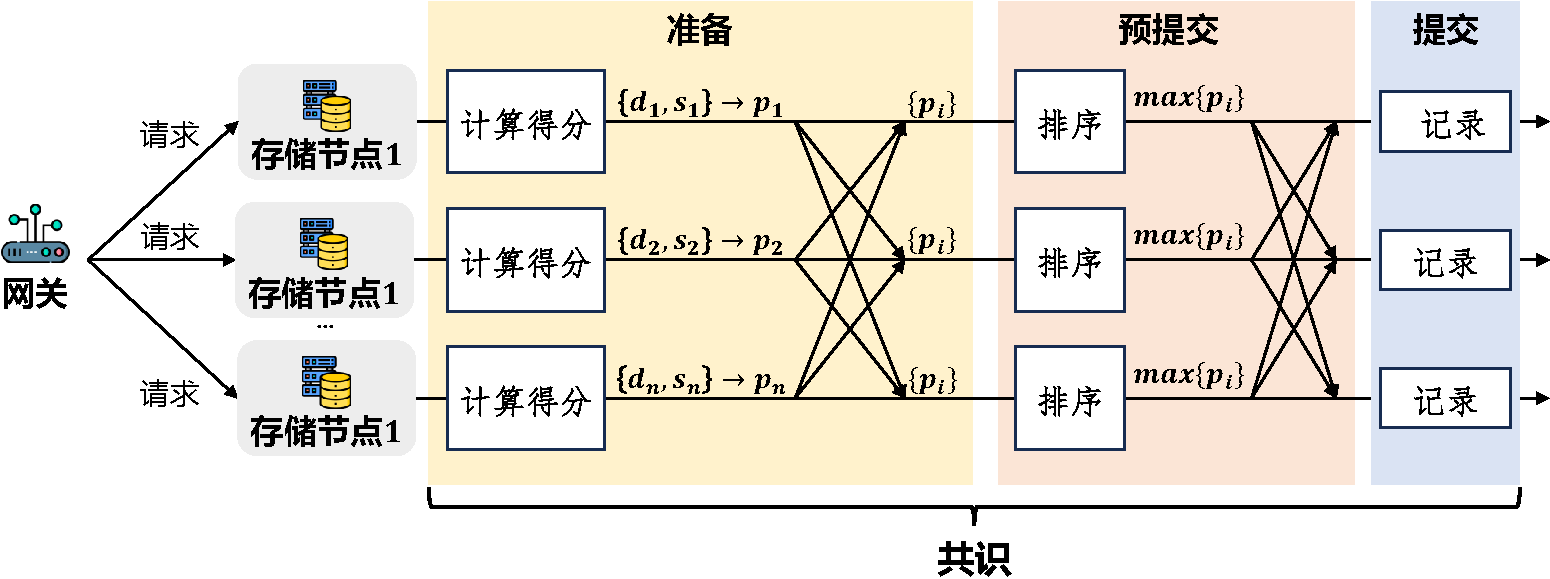
\includegraphics[width=1\linewidth]{figures/timechain/consensus.pdf}
    \caption{基于共识的节点选择机制工作流}
    \label{fig:consensus}
\end{figure}


\subsection{准备阶段}
在该阶段,每个节点通过考虑存储节点的距离、信誉等来计算分数,并将分数广播给所有其他节点。
TimeChain选择距离、剩余存储和存储质量作为指标,原因如下:
根据图\autoref{fig:dis_cdf},本文发现存储节点的距离会影响数据访问延迟。
因此,本文选择距离作为一个重要的指标。
此外,受到FileCoin~\cite{bauer2022filecoin}的启发,剩余存储空间和存储质量也是选择存储节点的重要因素。
剩余存储空间可以直接影响存储提供商的服务能力,而存储质量可以影响数据的完整性。
第$i$个节点的得分计算公式如下:

\begin{equation} 
    \label{eq:score}
    p_i=\alpha\cdot d_i+\beta\cdot s_i+\gamma\cdot q_i
\end{equation}

其中$d_i$表示第$i$节点和客户端节点之间的距离;$q_i$表示存储服务质量,可以从链上的服务记录中评估;$s_i$表示节点的剩余存储空间。
所有这些数据都可以在链上找到。
$\alpha$、$\beta$和$\gamma$是加权参数,这些系数可以根据特定的系统需求和性能要求进行调整。
例如,可以增加的权重以优先考虑存储完整性,而可以调整的权重以降低延迟。

\subsection{预提交阶段}
在本阶段,共识节点从其他节点接收准备好的消息集$\{p_i\}$。
当此节点的计时器超时并且收到超过$2f+1$个PREPARE消息时,共识节点根据它们收到的信誉优先级$\{p_i\}$决定最佳存储提供者。
如果每一轮共识只返回最近的节点,由于距离对信誉计算机制的影响,一些较近节点的存储压力可能会非常高。
为了平衡负载,共识节点将返回一组信誉最高的$n$节点,供网关随机选择,而不是信誉最高的节点。

为了防止恶意节点在\textbf{准备}阶段中的欺诈行为,在\textbf{预提交}阶段,共识节点的排序过程也需要对源节点的计算过程进行验证。
每个共识节点首先会对所有节点的信誉进行排序。
然后,共识节点会根据信誉由高到低的顺序,逐个验证节点的计算过程是否可信。
如果发现某个节点的计算过程不可信,共识节点将忽略该节点的信誉,继续验证下一个节点。
当共识节点收到的信誉最高的$n$个节点的信誉时,共识节点将这些节点返回给网关。

\subsection{提交阶段}
在\textbf{提交}阶段,所有节点都将收到其他节点推荐的最佳存储决策。
当相同的预提交消息的数量超过$f+1$时,此节点将向网关提交最佳存储节点集,由网关来决定最终的存储节点。
由于该网络中最多存在$f$个恶意节点,因此在\textbf{提交}阶段,虚假信息的数量一定少于诚实信息,所以该系统并不会受到恶意节点的威胁。

\section{共识过程的安全性分析}
本文在这里考虑这一共识协议的安全性。
由于TimeChain的共识协议只是基于PBFT添加了额外的信息,本文只考虑\textbf{准备}和\textbf{预提交}阶段额外信息带来的安全风险。

在\textbf{准备}阶段,如果一个节点伪造了自己的分数,网关可以很容易地检查分数的真实性,因为评估数据源都可以在链上找到。
一旦节点伪造了其信誉,该行为也将被记录在链上,从而影响下一次的信誉评估。
此外,由于最后只选择了一个存储节点,网关不关注所有节点得分的真实性,只关注所选节点的得分。

在\textbf{预提交}阶段,如果任何节点伪造了最终得分,则不会影响最终结果。
这是因为对于包含$f$拜占庭节点的$3f+1$节点的网络,必须在\textbf{提交}阶段获得相同的结果。

\section{本章小结}
本章专注于TimeChain中存储节点选择模块。
根据前文的测试分析可发现,存储节点与网关之间的距离直接影响数据访问延迟,而存储节点的可靠性则关乎数据的完整性和安全性。
因此,本章提出了一种基于共识协议的节点选择机制,该机制综合考虑了节点间的距离和历史服务记录,以全面评估存储节点的优劣。

本章分析了现有系统如Storj、CoopEdge和PipeEdge的局限性,指出它们依赖于集中式的节点选择服务,存在单点故障的风险。
为了解决这一问题,本章将节点选择过程与共识机制紧密结合,提出了一种新的节点选择算法。
该算法包括请求、准备、预提交、提交和回复五个阶段,通过这一流程,本章能够在确保安全性的同时,选择出最佳的存储节点。

在安全性分析中,本章证明了所提出的共识协议在PBFT基础上增加的信息并未引入额外的安全风险,因此该机制是安全的。
本章的共识协议考虑了准备阶段和预提交阶段的安全性,确保即使在存在恶意节点的情况下,系统也能正确选择出最佳的存储节点。
